
Dire~\cite{Hoche:2015sya}.  PFN~\cite{Komiske:2018cqr}.

Here, we will discuss now useless triple-collinear corrections to Dire were, and
how awesome double-soft contributions are.

\dots some Dire bullet points
\begin{itemize}
\item parton showers serve two purposes: $1)$ the distribution of low-multiplicity
(hard-scattering) states over states of arbitrarily high multiplicity, as well
as $2)$ generating the effect of resummation for observable depending only on 
low-multiplicity configurations.
\item these two purposes are often in conflict, e.g.\ choices to improve
$2)$ often limit the potential to improve $1)$ -- and vice versa. these
conflicts are not apparent at lowest (i.e.\ leading) order.
\item parton showers typically include states distributed with leading-order 
(leading-logarithmic) rate in their emission- and no-emission probabilities.
\item the rate of subsequent splittings is independent of the rate of
previous splittings, and the evolution scales at which splittings occur is
successively ordered -- such that resummation can occur.
\item with demand for more precise event generation, improved parton showers
are necessary. For example, the use of NLO PDFs (as e.g.\ mandated in NLO+PS
matching) in the parton shower in principle requires parton showers beyond
lowest order.
\item one way to improve the all-order behavior of the parton shower (point $2)$ 
above) while preserving a systematically improvable state distribution (point $1)$ 
above) is to consistently include higher-order and higher-multiplicity 
splitting functions in the parton shower.
\item several such configurations are shown in 
Figure~\ref{fig:jets:np:triplecollineardiagrams}. Such configurations are
already approximated through the iterated application of leading-order
splittings, albeit with incorrect rate (e.g.\ if the polarisation of 
the intermediate gluon in 
Figs.~\ref{fig:jets:np:triplecollineardiagrams1}-\ref{fig:jets:np:triplecollineardiagrams4},
\ref{fig:jets:np:triplecollineardiagrams7}-\ref{fig:jets:np:triplecollineardiagrams8}
is omitted, leading to an incorrect modulation of azimuthal angles,
or simply disregarding the interference between
$C_F$-type and $C_A$-type color structures from 
Figs.~\ref{fig:jets:np:triplecollineardiagrams7}-\ref{fig:jets:np:triplecollineardiagrams8})
or in a phase-space constrained by successive ordering (easily leading to the 
incorrect phase space volume, and thus failing to recover known anomalous
dimensions)
\item the correct final result is obtained by including the 
configurations~\ref{fig:jets:np:triplecollineardiagrams}
as new rates to the parton shower, and subtracting from these new rates
the leading-order result. This subtraction will, given a suitable definition
of the leading-order shower, act to ensure local finiteness of the new, 
subtracted, rates. We will call these subtracted rates ``corrections".
\item In~\cite{Hoche:2017iem}, triple-collinear corrections from diagram
similar to~\ref{fig:jets:np:triplecollineardiagrams2} were considered, with
the difference that instead of the primary parton (indicated with a double 
line), one of the quarks in the loop was considered as ``hard". Such
configurations give, upon integration, give rise to the flavor-changing 
DGLAP kernels $P_{qq'}$ and $P_{q\bar q}$. We
will call this ``triple-collinear" correction.
\item \cite{Dulat:2018vuy} considered all the 
diagrams~\ref{fig:jets:np:triplecollineardiagrams}
in the soft limit, and included all necessary virtual corrections obtained
by moving the cuts in the indiviual diagrams in all possible ways. We
will call this ``double-soft" correction.
\item It should be noted that there is overlap between the
triple-collinear and double-soft limits. A complete differential calculation 
that consistently (i.e.\ without overlap) includes all components has yet
to be produced. Thus, we assess the potential to find observables
that discriminate between leading-order and next-to-leading order
results separately for triple-collinear and double-soft corrections.
\item We find that the effect triple-collinear corrections (which integrate to
the DGLAP kernels $P_{qq'}$ and $P_{q\bar q}$) is difficult to pinpoint. 
It is somewhat surprising that the impact is almost vanishing.
\item We find that double-soft corrections have sizable impact, and can
easily be filtered out of the data. This is expected, since the theoretical
description of soft gluons changes significantly.
\item \emph{more to come, going to sleep now\dots}
\end{itemize}

\begin{figure}[h!]
\subfigure[blub]{
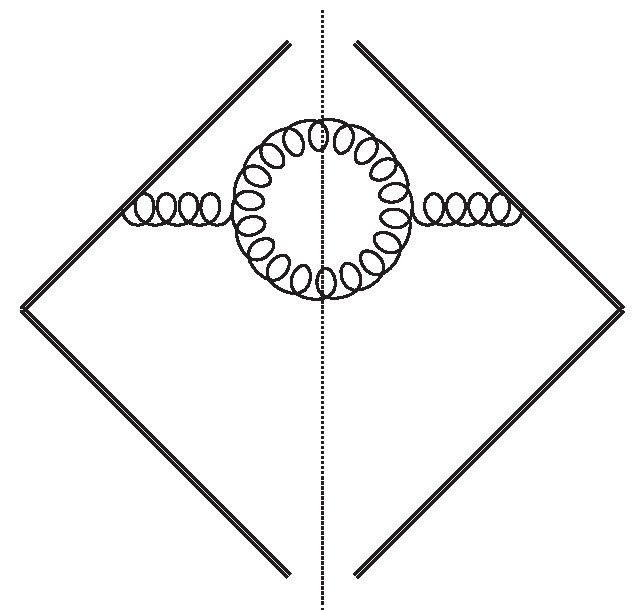
\includegraphics[width=0.23\textwidth]{figs/nlo_real_vpcg.pdf}
\label{fig:jets:np:triplecollineardiagrams1}
}
\subfigure[blub]{
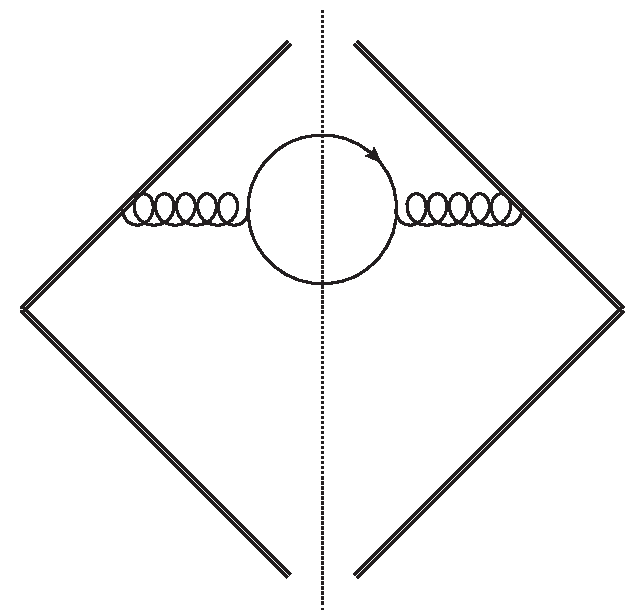
\includegraphics[width=0.23\textwidth]{figs/nlo_real_vpcq.pdf}
\label{fig:jets:np:triplecollineardiagrams2}
}
\subfigure[blub]{
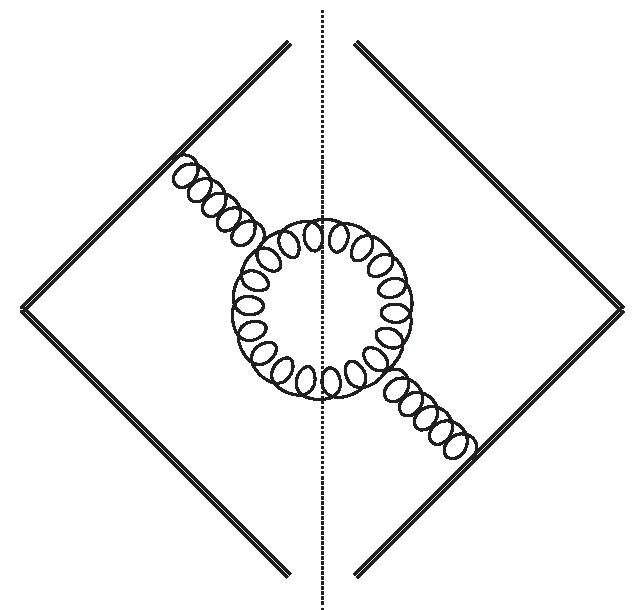
\includegraphics[width=0.23\textwidth]{figs/nlo_real_vpsg.pdf}
\label{fig:jets:np:triplecollineardiagrams3}
}
\subfigure[blub]{
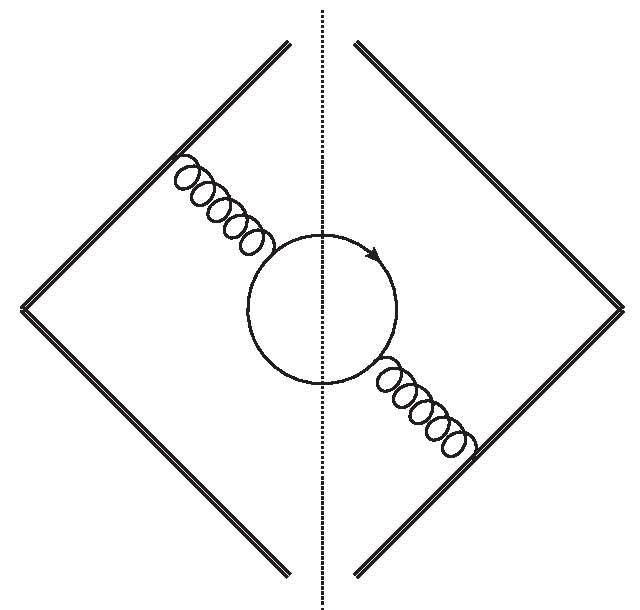
\includegraphics[width=0.23\textwidth]{figs/nlo_real_vpsq.pdf}
\label{fig:jets:np:triplecollineardiagrams4}
}
\\
\subfigure[blub]{
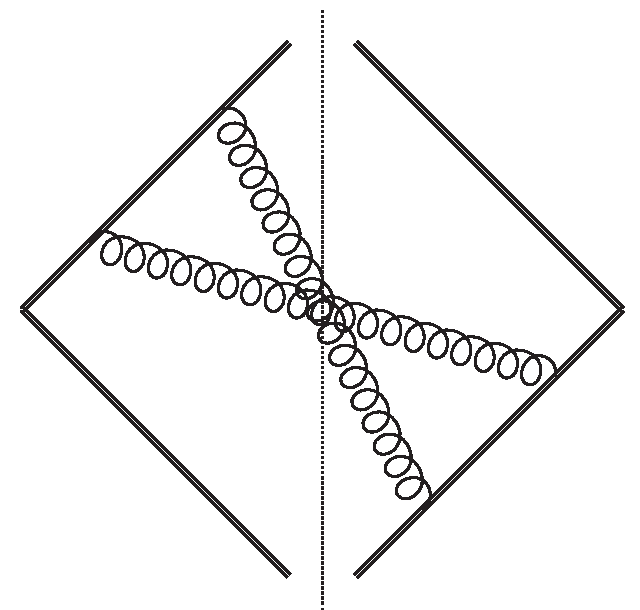
\includegraphics[width=0.23\textwidth]{figs/nlo_real_box1.pdf}
\label{fig:jets:np:triplecollineardiagrams5}
}
\subfigure[blub]{
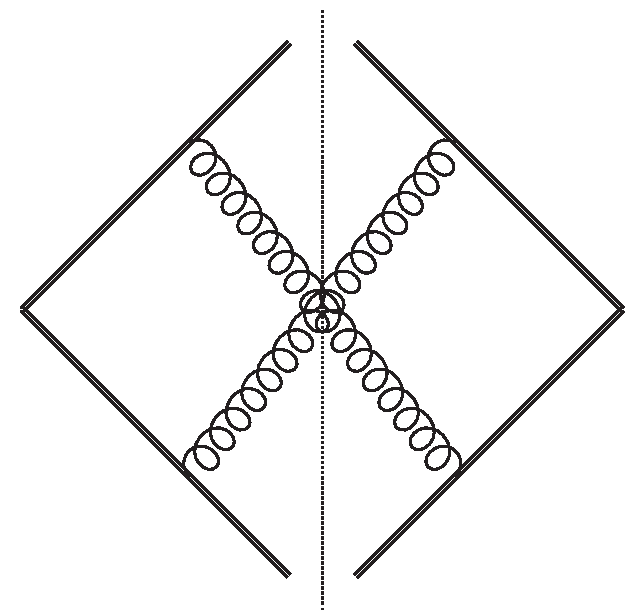
\includegraphics[width=0.23\textwidth]{figs/nlo_real_box2.pdf}
\label{fig:jets:np:triplecollineardiagrams6}
}
\subfigure[blub]{
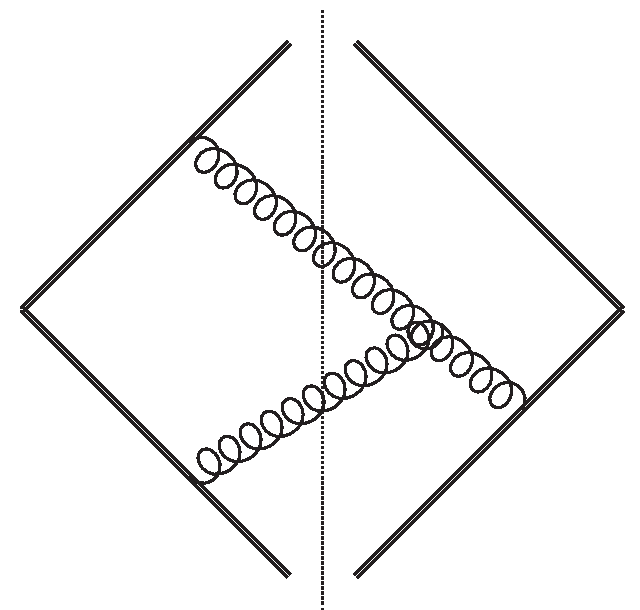
\includegraphics[width=0.23\textwidth]{figs/nlo_real_tgc1.pdf}
\label{fig:jets:np:triplecollineardiagrams7}
}
\subfigure[blub]{
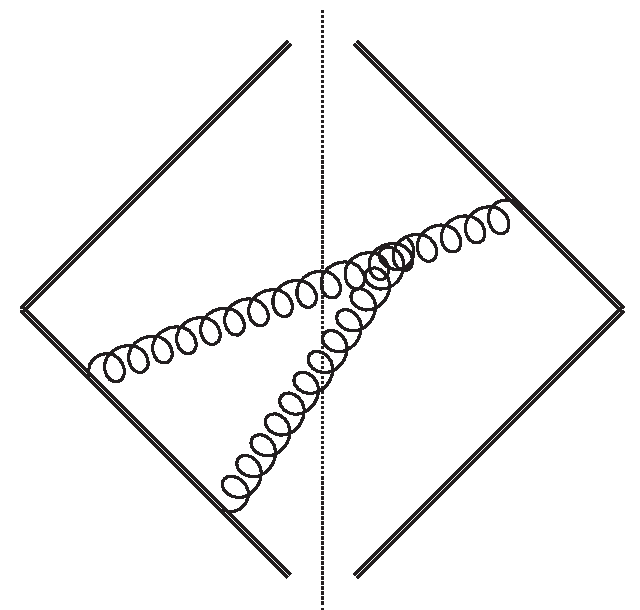
\includegraphics[width=0.23\textwidth]{figs/nlo_real_tgc2.pdf}
\label{fig:jets:np:triplecollineardiagrams8}
}
\caption{Replace me with proper diagrams!}
\label{fig:jets:np:triplecollineardiagrams}
\end{figure}

\begin{figure}[h!]
\centering
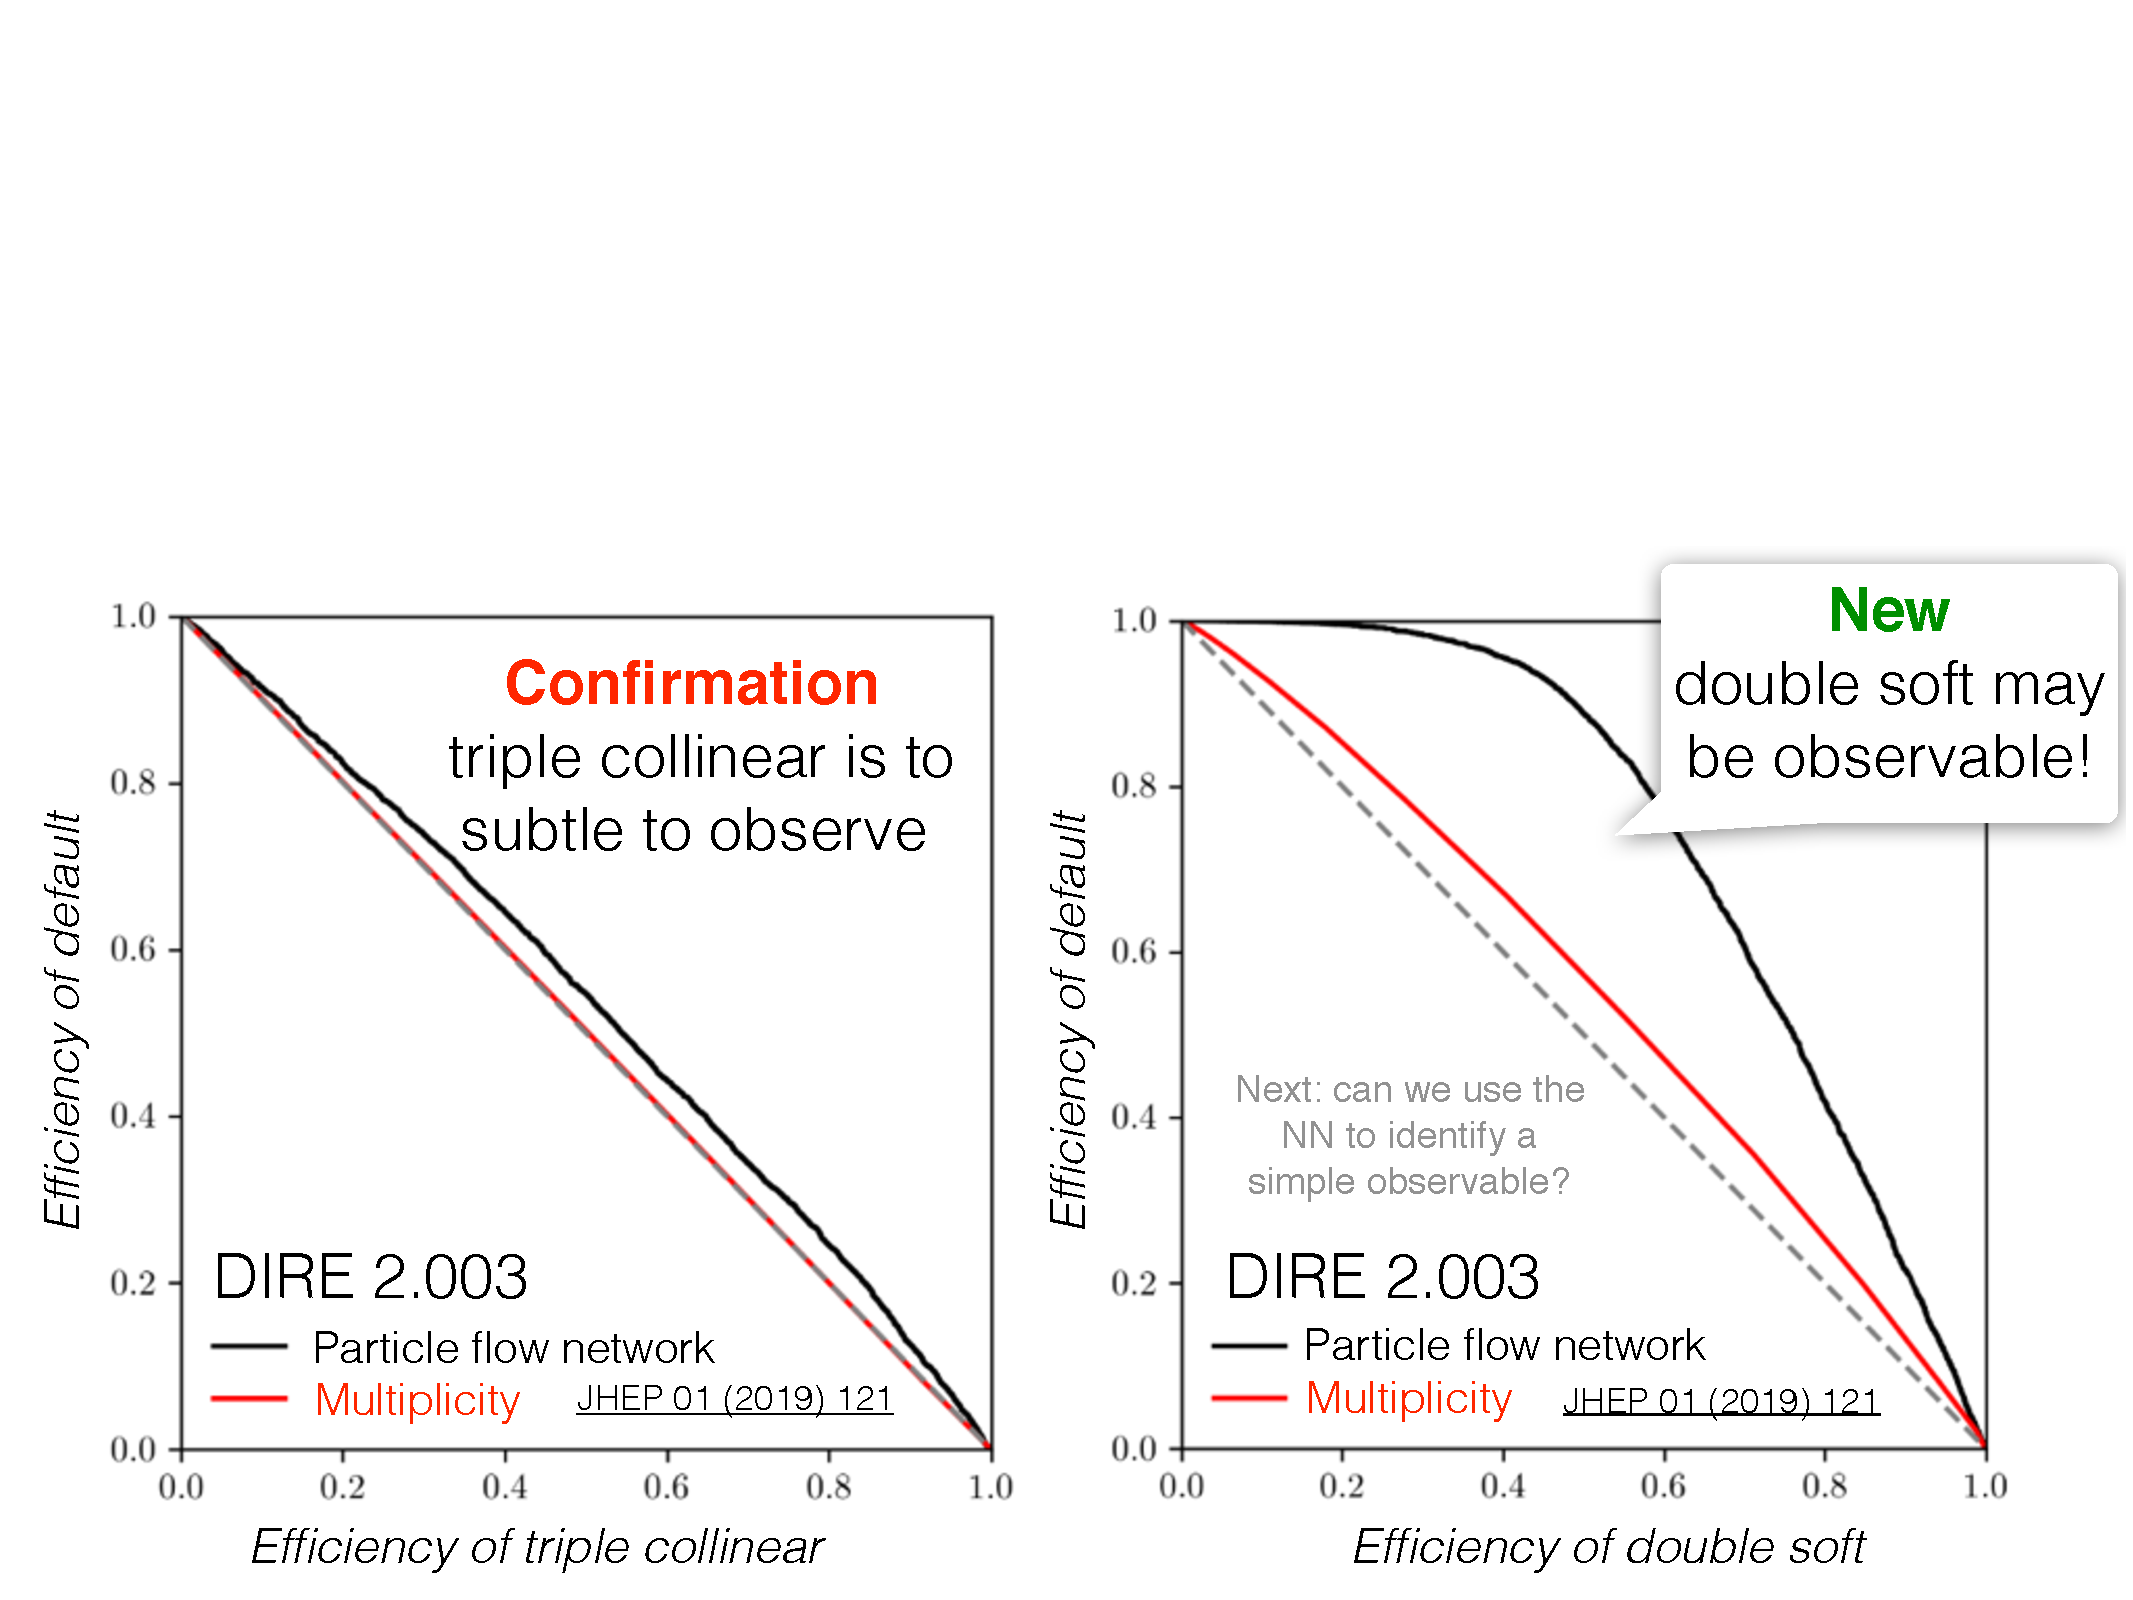
\includegraphics[width=0.85\textwidth]{figs/triplecollinear.pdf}
\caption{Replace me with proper plots!}
\label{fig:jets:np:triplecollinearNN}
\end{figure}




